\chapter{Subgradients}

Recall the definition of the (Frechet) derivative.

\begin{defn}[Frechet derivative]
    Let $f:X\rightarrow Y$. Then $f$ is (Frechet) differentiable at $x\in X$ if there exists a linear, continuous mapping $A:X\rightarrow Y$ such that 
    \begin{equation}
        \lim_{\|h\|\rightarrow 0}\frac{\| f(x+h) - f(x)  -Ah\|}{\|h\|}= 0.
    \end{equation}
    We denote $A=Df(x)$.
\end{defn}

\begin{defn}[Gradient]
    Let $f:X\rightarrow \R$ be differentiable with $X$ a Hilbert space. Then The gradient of $f$ at the point $x$, denoted as $\nabla f(x)$, is the unique element in $X$ such that 
    \begin{equation}
        Df(x)h =  \inner{\nabla f(x)}{h}, \quad h\in X.
    \end{equation}
    We denote $A=Df(x)$.
\end{defn}

The existence and uniqueness of the gradient is a direct consequence of the Riesz representation theorem since $Df(x)\in X^*$ if $f$ maps into the real numbers.
Note moreover, that \textbf{the gradient depends on the specific scalar product}.

While the above general definition might be a little abstract, in most cases we will be dealing with the gradient is quite simple. Specifically, whenever $X=\R^d$ equipped with the standard Euclidean scalar product, then 
\begin{equation}
    \nabla f(x) = Df(x)^T,
\end{equation}
\ie, the gradient is simply the transposed derivative.

We can interpret the derivative as the best linear approximation of the function at a point, that is,
\begin{equation}
    f(y) = f(x) + Df(x)(y-x) + o(\|y-x\|)
\end{equation}
where the small $o$ denotes a function tending to zero \emph{faster than linearly}. Most optimization methods can be interpreted as iteratively minimizing a easier approximation of the function. However, many functions of interest do not admit a gradient in the above sense, for instance we might want to solve problems of the form 
\begin{equation}
    \min\limits_x \frac{1}{2}\|Ax-b\|^2_2 + \lambda\|K x\|_1
\end{equation}
with $A$ and $K$ linear. These types of composite problems are extremely popular in imaging.
Thus, we may ask the question if it is possible to define a more general notion of a linear approximation which fulfills similar properties as the gradient. The next definition answers this question positively.

\begin{defn}[Subdifferential]
    Let $f:X\rightarrow Y$. We call $g\in X^*$ a subgradient of $f$ at $x\in X$ if 
    \begin{equation}
        f(x) + \langle g, y-x\rangle\leq f(y), \quad \forall y\in Y.
    \end{equation}
    The subdifferential $\partial f(x)$ at $x\in X$ is the set of all subgradients at $x$, \ie, 
    \begin{equation}
        \partial f(x) =\{ g\in X^*\;|\; f(x) + \langle g, y-x\rangle\leq f(y), \quad \forall y\in Y \}.
    \end{equation}
\end{defn}

Note, that the subdifferential might be empty. It is empty at every point $x\in X$ where $f(x)=\infty$. 

\begin{example}\
    \begin{enumerate}
        \item Norms: Let $f = \norm{\cdot}$, then
			\[
				\partial f(0) = \overline{B}_{\|\cdot\|_*, 1}(0),
			\]
            \ie, the unit ball of the dual norm.
            where we recall the definition of the dual norm $\|\cdot\|_*$
            \[
                \|y\|_* = \sup_{\|x\|\leq 1} \langle x,y\rangle.
            \]
			As an example, if \( f = \|\cdot\|_1\) on \( \R^n \), then
			\[
				\partial f(0) = \overline{B}_{||\cdot\|_\infty,1}(0) = [-1,1]^n.
			\]
        \item Given a nonempty set $S \subseteq X$ and a point $x \in S$, we consider the indicator function $\delta_S$. The subdifferential is given by
			\[
				\partial\delta_S(x)=\left\{y\in X^\ast:\inner{y}{z-x}\leq 0,\;\forall z\in S\right\}\eqqcolon N_S(x),
			\]
			which is the so-called \emph{normal cone} of $S$ at $x$.
			The subdifferential of the indicator function of the unit norm ball is given by
			\[
				N_{\overline{B}_{\|\cdot\|, 1}(0)}(x)=
				\begin{cases}
					\{y\in X^\ast|\|y\|_*\leq \inner{y}{x}\}&\text{if }\norm{x}\leq 1,\\
					\emptyset&\text{if }\norm{x}>1.
				\end{cases}
            \]
    \end{enumerate}
\end{example}


We want to make sure, that the subdifferential is, in fact, a generalization of the regular gradient:

\begin{lemma}
    Let $f:V\rightarrow \R$ be convex and differentiable at $x\in \dom(f)^\circ$. Then $\partial f(x) = \{\nabla f(x)\}$.
\end{lemma}
\begin{proof}
    In order to proof this result, we need to show (i) $\nabla f(x)\in \partial f(x)$ and (ii) if $g\in\partial f(x)$ then $g=\nabla f(x)$. The point (i) directly follows from the first order characterization of the gradient~\cref{convexity:thm:first_order}, which yields
    \begin{equation}
        f(x) + \inner{\nabla f(x)}{y-x}\leq f(y),\quad y\in V
    \end{equation}
    showing that $\nabla f(x)\in\partial f(x)$. For (ii) we note that by definition of the subgradient, for any $g\in\partial f(x)$, $h\in V$, and $t>0$ small enough such that $x+th\in\dom(f)$ we have
    \begin{equation}
        \inner{g}{h}\leq \frac{f(x+th)-f(x)}{t}.
    \end{equation}
    By letting $t\rightarrow 0$ it follows $\inner{g}{h}\leq \inner{\nabla f(x)}{h}$. Since this is true for all $h$, it follows $\inner{g}{h}= \inner{\nabla f(x)}{h}$ and, thus, $g=\nabla f(x)$.
\end{proof}
In fact, we also have the converse result, which we will not prove, however. That is, if the subdifferential is single-valued at a point $x$, then $f$ is differentiable in $x$ and $\partial f(x) = \{\nabla f(x)\}$.

\begin{figure}
    \centering
    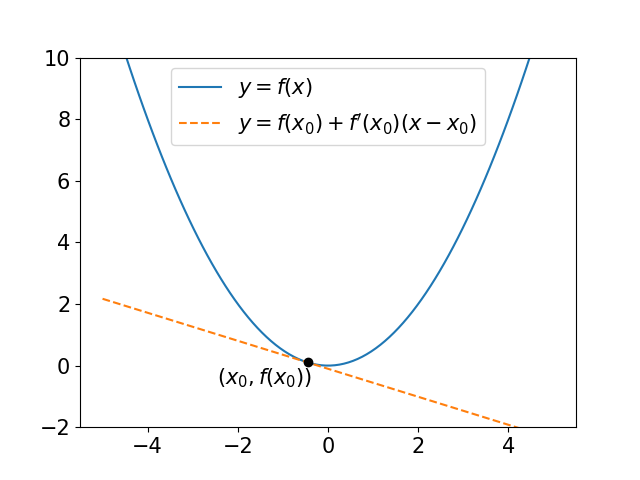
\includegraphics[scale=0.4]{figures/gradient}
    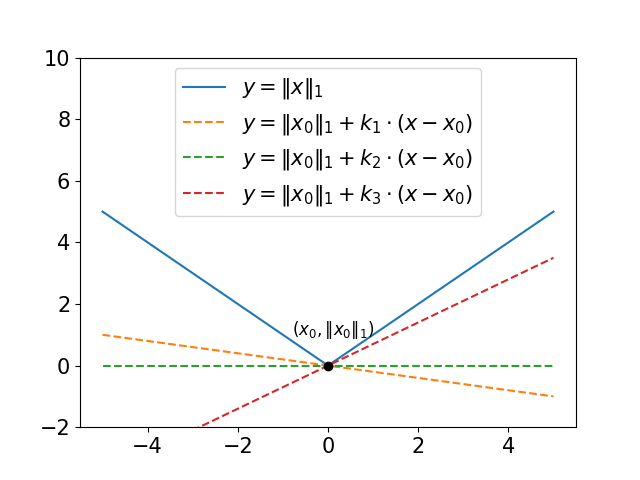
\includegraphics[scale=0.4]{figures/subgradient}
    \caption{Left: Illustration of the gradient as the slope of the tangent. Right: Illustration of the subgradient.}
\end{figure}

\begin{example}\
    \begin{enumerate}
        \item For $f(x)=\|x\|_2$ it follows
        \[
            \partial f(x) 
            = \begin{cases}
                \{\frac{x}{\|x\|_2}\}\quad& x\neq 0\\
                \overline{B}_{\|\cdot\|_2,1}(0)\quad&\text{else.}
            \end{cases}
        \]
        \item In particular, for $d=1$ and $f(x)=|x|$ it follows
        \[
            \partial f(x) 
            = \begin{cases}
                \{\sign(x)\}\quad& x\neq 0\\
                [-1,1]\quad&\text{else.}
            \end{cases}
        \]
    \end{enumerate}
\end{example}



\begin{lemma}
    If the domain of $f:X\rightarrow Y$ is convex and the subdifferential is nonempty at every point in the domain, then $f$ is convex.
\end{lemma}
\begin{proof}
    Let $x,y\in \dom f$, $\lambda\in (0,1)$ and $g\in \partial f(x+\lambda (y-x))$.
    By definition of the subdifferential we have
    \begin{gather}
        f(x+\lambda(y-x)) + \langle g, x - (x+\lambda(y-x))\rangle \leq f(x)\\
        f(x+\lambda(y-x)) + \langle g, y - (x+\lambda(y-x))\rangle \leq f(y)
    \end{gather}
    that is
    \begin{gather}
        f(x+\lambda(y-x)) + \langle g, -\lambda(y-x)\rangle \leq f(x)\\
        f(x+\lambda(y-x)) + \langle g, (1-\lambda)(y - x) \rangle \leq f(y).
    \end{gather}
    It follows
    \begin{equation}
        \begin{aligned}
            \frac{1}{\lambda} f(x+\lambda(y-x)) + \frac{1}{1-\lambda} f(x+\lambda(y-x))\leq \frac{1}{\lambda} f(x) + \frac{1}{1-\lambda} f(y).
        \end{aligned}
    \end{equation}
    Multyplying by $\lambda (1-\lambda)$ leads to 
    \begin{equation}
        \begin{aligned}
            f(x+\lambda(y-x)) \leq (1-\lambda) f(x) + \lambda f(y).
        \end{aligned}
    \end{equation}
\end{proof}


As stated above, the subdifferential may be empty. However, for convex functions we can guarantee the following:

\begin{theorem}\label{convexity:thm:nonempty_subgrad}
    Let $f:X\rightarrow\overline{\R}$ be proper and convex. Then $\partial f(x)\neq \emptyset$ for every $x\in \dom(f)^\circ$.
\end{theorem}
Before proving this result, we need some preperation:

\begin{lemma}
    The interior of a convex set is convex.
\end{lemma}
\begin{proof}
    Let $C$ be convex. If $C^\circ=\emptyset$ there is nothing to prove so assume $C^\circ\neq \emptyset$. 
    Let $x,y\in C^\circ$ and $\lambda\in (0,1)$. We have to show that $x_\lambda\coloneqq\lambda x + (1-\lambda)y\in C^\circ$.
    Then there exists $\epsilon$ such $B_\epsilon(x),B_\epsilon(y)\subset C^\circ$. Now let $z\in B_{\epsilon}(x_\lambda)$. That is, $z=x_\lambda + h$ with $\|h\|<\epsilon$. We may write
    \begin{equation}
        z = \lambda x + (1-\lambda)y + h = \lambda (x+h) + (1-\lambda)(y + h)
    \end{equation}
    and since $x+h\in B_\epsilon(x)\subset C$, $y+h\in B_\epsilon(y)\subset C$ it follows that $z\in C$ by convexity of $C$. Thus, $B_\epsilon(x_\lambda)\subset C$ and $x_\lambda\in C^\circ$ concluding the proof.
\end{proof}

\begin{lemma}
    If $C\subset\R^d$ is convex and $C^\circ=\emptyset$ then there exists a hyperplane $H$ such that $C\subset H$.
\end{lemma}
\begin{proof}
    We may assume without loss of generality $0\in C$. Otherwise, consider for any $x_0\in C$, $\tilde{C} = C-x_0$. 
    
    We will show that $C$ is a subset of a $d-1$ dimensional subspace. Assume to the contrary that $C$ contains $d$ linearly independent elements, \ie, there exist $x_1,\dots,x_d\in C$ which are linearly independent. By convexity, also the convex hull
    \begin{equation}
        \conv((x_i)_i)=\bigg\{ \sum_{i=1}^d\lambda_i x_i\;\bigg|\; \lambda\in \Delta^d\bigg\}
    \end{equation}
    is a subset of $C$. We claim that $\frac{1}{2d}\sum_{i=1}^d x_i\in C^\circ$. First note that by convexity
    \[
        \frac{1}{2d}\sum_{i=1}^d x_i = \sum_{i=1}^d \frac{1}{2d} x_i + \frac{1}{2}0 \in C.
    \]
    Note that, since the $x_i$ are linearly independent, we may write any $h\in\R^d$ as $h=\sum_i \lambda_i x_i$. Indeed, the mapping $\lambda\mapsto h$ is a bijective linear mapping $\R^d\rightarrow\R^d$. Therefore, there exists $\epsilon>0$ such that if $\|h\|<\epsilon$ it follows $|\lambda_i|<\frac{1}{2d}$ for all $i$. In particular, we have $\frac{1}{2d} + \lambda_i \in [0,1]$ and $\sum_{i=1}^d (\frac{1}{2d} + \lambda_i)\in [0,1]$.
    As a consequence, for any $\|h\|<\epsilon$ we find
    \begin{equation}
        x+h = \sum_{i=1}^d \big(\frac{1}{2d} + \lambda_i\big) x_i = \sum_{i=1}^d \big(\frac{1}{2d} + \lambda_i\big) x_i + \bigg(1 - \sum_i\big(\frac{1}{2d} + \lambda_i\big) \bigg)0\in C.
    \end{equation}
    Therefore, if $C$ contained $d$ linear independent elements, its interior would not be empty as $B_\epsilon(0)\subset C$. Thus, $C$ contains at most $d-1$ linearly independent elements, say $x_1,\dots,x_{d-1}$. In particular, 
    \[
        C\subset \span \{ x_i\;|i=1,\dots,d-1\}
    \]
    concluding the proof.
\end{proof}
Using the two previous results we can prove the supporting hyperplane theorem.
\begin{theorem}[Supporting hyperplane theorem]
    Let $C\subset V$ be nonempty and convex and $x_0\in \partial C = \overline{C}\setminus(C^\circ)$\footnote{the boundary of $C$}. Then there exists $a\in V^*$, $a\neq 0$ such that
    \begin{equation}\label{subgradient:eq:supporting}
        \inner{a}{v}\leq \inner{a}{x_0},\quad v\in C.
    \end{equation}
\end{theorem}
\begin{proof}
    We consider only the finite dimensional case.
    The result is a direct consequence of Hahn-Banach's separation theorem. We make a case distinction. Assume first, $C^\circ\neq \emptyset$. Then $C^\circ$ is open, convex, and non-empty. We may apply Hahn-Banach separation theorem to the sets $C^\circ$ and $\{x_0\}$ yielding the result. In the converse case, if $C^\circ$ is empty, then $C$ is contained in an affine subset $H$ of at most dimension $d-1$. This affine subset also contains $x_0$ by closedness. Let $a\in V^*$ and $b\in \R$ such that 
    \[
        H=\{x\;|\; \inner{x}{a} = b\}.
    \]
    Then this $a$ satisfies~\eqref{subgradient:eq:supporting}.
\end{proof}

We can now prove existence of a subgradient.

\begin{proof}[Proof of \cref{convexity:thm:nonempty_subgrad}]
    We want to show that there exists $g\in X^*$ such that
    \begin{equation}
        f(x)+\inner{g}{y-x}\leq f(y)
    \end{equation}
    for all $y\in X$. This is equivalent to showing that
    \begin{equation}\label{subgrad:eq:nonempty_subdiff1}
        \inner{g}{y} - f(y)\leq \inner{g}{x} - f(x).
    \end{equation}
    This already looks quite similar to the structure of Hahn-Banach. In order to be able to use it, we switch to the epigraph. Note that $(x,f(x))\in \partial \epi(f)$. Moreover, by convexity of $f$, $\epi(f)$ is convex as well. We can therefore apply the supporting hyperplane theorem and find an element $(g,-\alpha)\in (V\times\R)^* = V^*\times\R$ such that\footnote{writing it as $-\alpha$ is just for convenience as we will see in a few seconds}
    \begin{equation}\label{subgrad:eq:nonempty_subdiff2}
        \inner{(g,-\alpha)}{(y,t)}\leq \inner{(g,-\alpha)}{(x,f(x))},\quad (y,t)\in \epi(f).
    \end{equation}
    which is equivalent to
    \begin{equation}
        \inner{g}{y}-\alpha t \leq \inner{g}{x} - \alpha f(x),\quad (y,t)\in \epi(f).
    \end{equation}
    We want to show now, that $\alpha>0$. Assume $\alpha<0$. Since $(x,t)\in \epi(f)$ for any $t>f(x)$ we may let $t\rightarrow \infty$ leading to a contradiction. Now assume next that $\alpha=0$. This would imply 
    \begin{equation}
        \inner{g}{y-x} \leq 0
    \end{equation}
    for all $y\in\dom(f)$ and therefore, since $x\in \dom(f)^\circ$, $g=0$. Since Hahn-Banach provides a non-trivial \emph{separating element} we also have a contradiction. Therefore, $\alpha>0$ and we may divide~\eqref{subgrad:eq:nonempty_subdiff2} by $\alpha$ to obtain
    \begin{equation}
        \inner{\tilde{g}}{y} - t \leq \inner{\tilde{g}}{x} - f(x),\quad (y,t)\in \epi(f).
    \end{equation}
    with $\tilde{g} = g/\alpha$. Picking $t=f(y)$ it follows that $\tilde{g}\in\partial f(x)$ and concluding the proof.
\end{proof}


Similar to the case of the regular derivative, in order to compute subgradients in practice, we can derive several computation rules.


\begin{theorem}
    Let $f:V\rightarrow\R$ proper and convex and $\alpha\geq 0$. Then for any $x\in\dom(f)$ we have
    \[
        \partial(\alpha f)(x) = \alpha\partial f(x).
    \]
\end{theorem}
\begin{proof}
    Exercise.
\end{proof}

\begin{theorem}
    Let $f,g:V\rightarrow\R$ be proper and convex. Then for any $x\in\dom(f)\cap\dom(g)$ we have
    \[
        \partial f(x) + \partial g(x)\subset \partial (f+g).
    \]
    Moreover, if there exists an $x_0\in \dom(f)^\circ \cap\dom(g)$ then
    \[
        \partial f(x) + \partial g(x) = \partial (f+g).
    \]
\end{theorem}
\begin{proof}
    We only proof the first inclusion. The proof of the second one is a little more involved and relies on the Hahn-Banach separation theorem similar to the proof of existence of subgradients.

    Assume $p_1\in \partial f(x)$ and  $p_2\in \partial g(x)$, that is
    \begin{equation}
        \begin{aligned}
            f(x) + \langle p_1, y-x\rangle&\leq f(y)\\
            g(x) + \langle p_2, y-x\rangle&\leq g(y)
        \end{aligned}
    \end{equation}
    Adding both inequalities yields
    \begin{equation}
        \begin{aligned}
            f(x)+ g(x) + \langle p_1+p_2, y-x\rangle \leq f(y) + g(y)
        \end{aligned}
    \end{equation}
    so that $p_1+p_2\in \partial (f+g)(x)$.
\end{proof}

Finally, we list some more \emph{computation rules} for the subdifferential without proof.
\begin{theorem}
    Let $f:W\rightarrow\Rb$ be a proper, convex, and lower semi-continuous function and $A:V\rightarrow W$ a linear transformation.
    Define $h(x)=f(Ax+b)$ with $b\in W$. For any $x\in\dom(h)$ (weak rule)
    \[
        A^\ast(\partial f(Ax+b))\subseteq\partial h(x).
    \]
    with equality if there exists $x_0\in \dom(h)^\circ$ (strong rule).
\end{theorem}

The derivative of a composition of differentiable functions is computed by using the chain rule, \ie, the derivative of the function $h(x) = g(f(x))$ is given by $D h(x) = Dg(f(x))Df(x)$.
This formula can be extended to the subdifferential calculus:
\begin{theorem}
    Let $f:V\rightarrow \R$ be a convex function, $g:\R\rightarrow \R$ be a non-decreasing convex function and $h=g\circ f$.
    Further, let $x\in V$ and suppose that $g$ is differentiable at the point $f(x)$.
    Then,
    \[
        \partial h(x)= g'(f(x))\partial f(x).
    \]
\end{theorem}

\begin{theorem}
    Let $f:V\to(-\infty, \infty]$ be a proper convex function. Then
    \[
        x^\ast\in\arg\min_{x\in V} f(x)
    \]
    if and only if $0\in\partial f(x^\ast)$.
\end{theorem}
\begin{proof}
    The proof directly follows from the subgradient inequality
    \[
        f(x)\geq f(x^\ast)+\inner{0}{x-x^\ast}
    \]
    for any $x\in\dom f$.
\end{proof}

\begin{theorem}
    Let $f:V\rightarrow(-\infty,\infty]$ be a proper and convex function and $C\subseteq V$ be a convex set for which $\dom(f)^\circ\cap C^\circ \neq\emptyset$.
    Then $x^\ast\in C$ is a solution of the constrained optimization problem if and only if
    there exists $g\in \partial f(x^\ast)$ such that
    \[
        \inner{g}{x-x^\ast}\geq 0
    \]
    for all $x\in C$.
\end{theorem}


